\documentclass[11pt]{jsarticle}

\usepackage{SPR}

\headerSPR
\begin{document}
	\titleSPR{\number\year}{\number\month}{\number\day}{D2}{吉田 皓太郎}
%%%%%%%%%%%%%%%%%%%%%%%%%%%%%%%%%%%%%%
	\articleSPRabst
		\begin{itemize}
			\item 機械学習を用いたカップ形状の設計支援
			\item 着後形状予測のためのカップの変形解析
		\end{itemize}
		
		
	\articleSPRobj
		\begin{enumerate}
			\item 定性的な機能要求を満たせるようなカップ形状を設計できる
			\item 布の物性とカップのパターンがどのような結びつきを持っているかを調べることができる.
		\end{enumerate}
%%%%%%%%%%%%%%%%%%%%%%%%%%%%%%%%%%%%%%
% 1.前回からのノルマ
	\articleSPRitemsone
		%\begin{enumerate}
		%	\item A
		%\end{enumerate}
		
		\tableofcontents
		
		
%%%%%%%%%%%%%%%%%%%%%%%%%%%%%%%%%%%%%%
%\begin{itemize}
%	\item 新規手法について
%	\item ISFAアウトライン
%\end{itemize}
%%%%%%%%%%%%%%%%%%%%%%%%%%%%%%%%%%%%%%
% 2.具体的な成果
	\articleSPRitemstwo
	\renewcommand{\labelitemi}{$\blacktriangledown$}
	%\renewcommand{\labelitemi}{$\bigcirc$}
	\newcommand{\argmax}{\mathop{\rm arg~max}\limits}
	\newcommand{\argmin}{\mathop{\rm arg~min}\limits}
	\newcommand{\Ker}{{\rm Ker}}
	\newcommand{\rank}{{\rm rank}}
%%%%%%%%%%%%%%%%%%%%%%%%%%%%%%%%%%%%%
	\section{研究進捗について}
		\subsection{研究会進捗}
			$ \bd{y} = \bd{K}\bd{a} $とおき,$ \bd{a}^T \bd{K} \bd{a} / \lambda_{\min} - 1 $を制約を置く.これにより,桁数の小さい誤差も対応できるようにしている.(ここらへんは誤差評価の仕方に工夫のし甲斐があるかもしれない)
			
			計算結果を示す.制約に関してはそれぞれ数$ \% $程度の誤差にはなったものの,対応する出力値$ \phi_1 \frac{V}{S} $を比較すると,@@と@@であり,誤差の広がりが認められる.また,主に固有値が小さい$ D $の値に関して,誤差が広がっている形となっている.
			\bfig[H]
				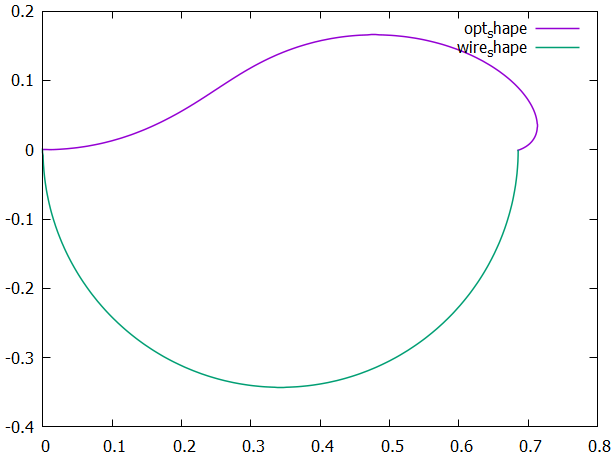
\includegraphics[scale = 0.5]{./figure/AlignWire_xyview.png}
			\efig
			
			\bfig[H]
			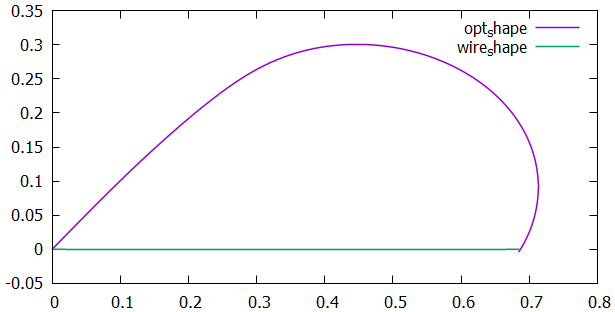
\includegraphics[scale = 0.5]{./figure/AlignWire_xzview.png}
			\efig
			
			\bfig[H]
			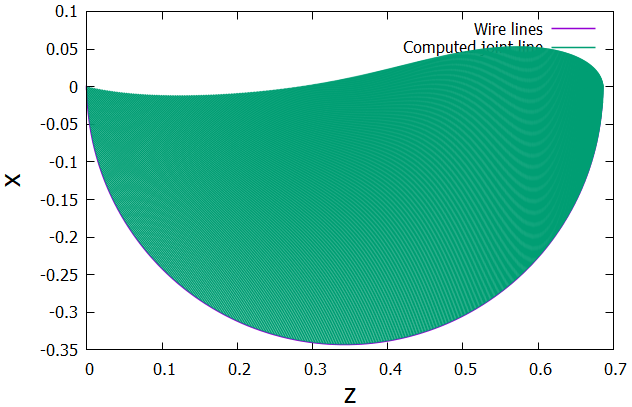
\includegraphics[scale = 0.5]{./figure/ObtainedRidgeLinefromz-x.png}
			\efig
			
			\bfig[H]
			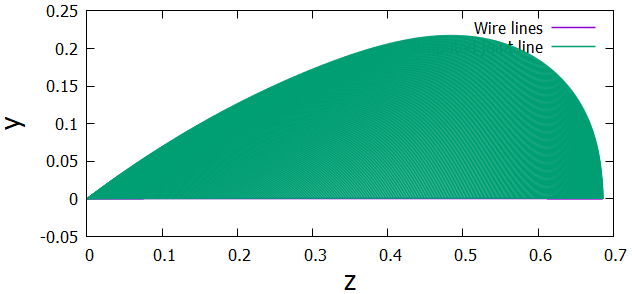
\includegraphics[scale = 0.5]{./figure/ObtainedRidgeLinefromz-y.png}
			\efig
		\subsection{論文調べ}
			可展面関係の論文で,気になった論文がありました.この論文では,自由に引かれた二つの曲線を微修正し,可展面条件を満たすように最適化することが行なわれておりました.
		\subsection{設計工学特集号の案内}
			前回の設計工学部門において,特集号の投稿依頼がきました.追記内容として,もしかして使えるかもしれない?理論の追記事項を上げておきます.
			\section{曲面論の基本定理など}
	\subsection{曲面論の基本定理の成立条件について}
		曲線論の基本定理は,曲率$ \kappa $および捩率$ \tau $が与えられる場合,曲線は回転・平行移動を除いて一意に決定されるという定理であった.この基本定理は,フレネ・セレの公式からも明らかである.
		
		一方,曲面論における基本定理は,曲面の第一基本形式および第二基本形式が与えられる場合,その曲面が一意に決定できるというものである.この基本定理の成立条件は
		
		\begin{eqnarray}\label{eq:SurfaceConds}
			K &=& \det \{ b_{ij} \} \\
			b_{i2,1} &=& b_{i1,2}
		\end{eqnarray}
		が成立することである.ただし,$ \{ a_{ij}\} $は,$ a_{ij} $を成分に持つ行列全体を表す.この$ b $に関しては,曲面に関する係数だが,これについては外微分形式を導入したのち,説明する.
		
		我々が定式化した曲面モデルが,上記の2式を満たすことを証明する.
	\subsection{数式のおことわり}
		本式において,$ R^n $は$ n $次元ユークリッド空間を表し,その座標を$ \bd{x} = \{ x_i\}_{i=0,\cdots , n-1} $と表す.$ \{ a_{ij}\} $は,$ a_{ij} $を成分に持つ行列全体を表す.また,行列式は$ \det A $のように表す.また,当研究室において用いられていた主曲率方向$ \bd{d}_1,\bd{d}_2 $や物体標構の各軸回転率,母線角はそれぞれ同様のものを用いるとする.
	
	\subsection{多様体および外微分形式の導入の概説}
		$ n $次元空間における$ n $次元多様体とは,空間$ M $と局所座標近傍の系$ \{U_i\}_{i=0,\cdots ,N} $からなり,特に$ n $次元微分可能多様体は,次の定義を満たす.
		\begin{itemize}
			\item $ M $は位相空間(点の近傍が定義可能な空間)である.
			\item $ M $は開集合の族$ \{ U_j \} $と,各$ U_j $から$ R^n $への写像$ \phi_j(U_j) $を持つ.
			\item $ \{ U_j \} $は$ M $を覆う.すなわち,$ \cup_j  U_j  = M$
			\item $ \{ \phi_j | U_j \rightarrow R^n\} $は,開集合で,$ \phi_j $は,$ U_j $から$ \phi_j (U_j) $上の同相写像である.
			\item $ U_j \cap U_i \neq 0$となる$ i,j $の組に対して,$ \phi_i(U_i \cap U_j) $から,$ \phi_j(U_i \cap U_j) $への写像$ \phi_j \circ  \phi_i^{-1} $は,無限回微分可能である.
		\end{itemize}
		上記の内,(2)~(5)を満たす族$ \{ U_j,\; \phi_j\} $を座標近傍系といい,個々の要素を座標近傍という.
		
		多様体上の微分を考えるにあたって,微分積分における外積$ \wedge $を次のような性質を満たす演算と定義する.
		\begin{itemize}
			\item 分配則$ (\bd{x}_1 + \bd{x}_2) \wedge \bd{y} = \bd{x}_1 \wedge \bd{y} + \bd{x}_2 \wedge \bd{y} $
			\item 結合則$ \bd{x} \wedge (\bd{y} \wedge \bd{z}) = (\bd{x} \wedge \bd{y} )\wedge \bd{z}$
		\end{itemize}
		また,空間基底$ \{ \bd{\sigma}_i \} $に対し,$ \bd{a} = \sum a_i \bd{sigma}_i,\bd{b} = \sum b_j \bd{\sigma}_j$と表されるベクトル集合を,1-ベクトルと呼び,外積によって定義される次のような空間
		\begin{equation}\label{eq:Gaiseki}
			\bd{a} \wedge \bd{b} = \sum_i \sum_j a_i b_j (\bd{sigma}_i \wedge \bd{sigma}_j)
		\end{equation}
		によって得られるベクトルを2-ベクトルと呼ぶ.これを一般化すると$p$-ベクトルは,次式のように表される.
		\begin{equation}\label{eq:Gaiseki2}
			\sum_{i_1,\cdots i_p} a_{i_1,\cdots,i_p} (\bd{sigma}_1 \wedge \cdots \wedge \bd{sigma}_n)
		\end{equation}
		$ p $-ベクトル$ \mu $および$ q $-ベクトル$ \nu $に対し,外積は次のような性質を持つ.
		\begin{equation}\label{eq:Gaiseki3}
			\mu \wedge \nu = (-1)^{pq} \nu \wedge \mu
		\end{equation}
		$ R^n $上の$ n $次元微分可能多様体$ M $において,多様体上のある点$ P $における1次外微分形式を1-形式と呼び,$ \sum a_i(P)dx_i $と定義する.次式を,点$ P $における$ p $次微分形式と呼び,$ p $-形式と表す.
		\begin{equation}\label{eq:BIBUN1}
			\sum_{h_1} \cdots \sum_{h_p} a_{h_1,\cdots,h_p} dx_{h_1} \wedge \cdots \wedge dx_{h_p}
		\end{equation}
		外微分作用素$ \Delta $は,$p$-形式を$ (p+1) $-形式にする線形写像であり,次の性質を持つと定義する.
		\begin{itemize}
			\item $ \Delta(\omega + \eta) = d\omega + d\eta $ 
			\item $ \lambda $が$ p $-形式の場合において,$ \Delta(\lambda \wedge \mu ) = \Delta \lambda \wedge \mu + (-1)^p \lambda \wedge \Delta \mu $
			\item $ \Delta (\Delta \omega) = 0 $
			\item 関数$ f $に対して$ \Delta f = \sum \frac{\partial f}{\partial x_i }\Delta x_i $
		\end{itemize}
	\subsection{曲面における外微分形式}
		曲面の全体は$ n=2 $の場合における多様体として考えることができる.曲面$ M $において,各点で接平面内のベクトル$ \bd{e}_1,\bd{e}_2 $を
		\begin{equation}\label{eq:e1e2}
			\bd{e}_1 \cdot \bd{e}_1 = \bd{e}_2 \cdot \bd{e}_2 = 1, \;\; \bd{e}_1 \cdot \bd{e}_2  = 0
		\end{equation}
		となるように選び,$ \bd{e}_3 = \bd{e}_1 \times \bd{e}_2 $となるように定める.この$ \bd{e}_3 $は曲面に対する法線ベクトルと符号を除いて一致する.以降では,曲面に対する法線ベクトルと一致すると仮定する.
		点$ \bd{r} $が曲面上に沿って移動するとき,その変化量は
		\begin{equation}\label{eq:dreq}
			\Delta \bd{r} = \sigma_1 \bd{e}_1 + \sigma_2 \bd{e}_2
		\end{equation}
		と表すことができる.この$ \sigma_i \;(i=1,2) $は1-形式であり,2-形式$ \sigma_1 \wedge \sigma_2 $は面積要素を表す.
		
		また,$ \bd{e}_j $は正規直交基底の性質を満たすため,
		\begin{equation}\label{eq:de_jeq}
			\Delta \bd{e}_i = \sum_j \omega_{i,j} \bd{e}_j
		\end{equation}
		と書ける.1-形式$ \omega_{i,j} $は,次式の性質を満たす.
		\begin{equation}\label{eq:omega_ijeq}
			\omega_{i,j} = - \omega_{j,i},\;\; \omega_{i,i} = 0
		\end{equation}
		$ \Delta (\Delta \bd{r}) = \bd{0} $より
		\begin{equation}
			\Delta \bd{e}_i = \sum_j \sigma_j \wedge \omega_{j,i}\;\;(i=1,2) 
		\end{equation}
		\begin{equation}\label{eq:FirstFundamentalEq}
			\bd{e}_1 \cdot \bd{e}_1
		\end{equation}
		を得る.式(\ref{eq:FirstFundamentalEq})を第一構造式と呼ぶ.また,$ \Delta \Delta \bd{e}_i =\bd{0}$から,
		
		\begin{equation}\label{eq:d_omgEq}
			\Delta \omega_{i,k} = \sum_{j=1}^{3} \omega_{i,j} \wedge \omega_{j,k}
		\end{equation}
		を得る.
		また,式(\ref{eq:FirstFundamentalEq})より,$ \omega_{i,3} $は,$ b_{i,j} $を係数とし,$ \sigma_1,\sigma_2 $の線形結合によって次式で表現することができる.
		\begin{eqnarray}
			\omega_{i,3} = \sum_{j=1}^2 b_{i,j} \sigma_j
		\end{eqnarray}
		この$ b_{i,j} $を用いて,ガウス曲率は$ K=\det \{b_{i,j}\} $と表すことができる.また,$ \Delta \omega_{2,1} = K \sigma_1 \wedge \sigma_2  $が成立し,これを第二構造式という.
		$ \Delta \omega_{i,3} - \sum_{j=1}^{3} \omega_{i,j} \wedge \omega_{j,3} = 0 $より,
		\begin{equation}\label{eq:DeltaBeq}
			\sum_{k=1}^{2} (\Delta b_{i,k} - \sum_{j=1}^2 b_{i,j} \omega_{k,j} - \sum_{j=1}^2 b_{j,k} \omega_{i,j}) \wedge \sigma_k = 0
		\end{equation}
			\section{入力をなぜGPで表現したか}
			タイトルの件について,おそらく研究会の説明等では不足であると考え,追記します.
			
			この表現の目的はある関数$ f(x) $の特徴を記述するパラメータを入力パラメータとしたいと考えたところから出発します.最も単純で馴染みの深い方法としては,下記のように$ f(x) $を基底関数$ \bd{\phi} = \{ \phi_i(x) \} $の重み付き線形和によって表現する方法です.
			\begin{equation}\label{eq:LinearEq}
				f(x) = \sum_{i=0}^{N} w_i \phi_i(x)  = \bd{\phi} \bd{w}
			\end{equation}
			入力のデータセット$ \bd{x} = \{x_i\} $出力データセット$ \bd{\hat{f}} = \{\hat{f}_i\}$が与えられている場合,$ \bd{w} $は次のような二乗誤差を最小化することで得られる.
			\begin{equation}\label{eq:ErrorToMinimize}
				E =  \sum_{i=0}^{N} (\hat{f}_i - \sum_{j=0}^{N} w_j \phi_j(x_i))^2
			\end{equation}
			しかしこの場合,$ \dim(\bd{w}) $をどの程度であればよいのかは関数毎に設定が必要である点や,パラメータの次元が増加してしまう,などの問題があります.
			
			ガウス過程では,この$ \bd{w} $があるガウス分布$ \mathcal{N}(\bd{0},\lambda^2 \bd{I}) $から生成されたものと仮定します.この場合,出力の$ f $もまたガウス分布に従います.平均と分散はそれぞれ次式のように計算されます.
			\begin{equation}\label{eq:Avg}
				\bd{m} = \mathbb{E}(f(x)) = \bd{\phi} \cdot \mathbb{E}( \bd{w}) = \bd{0}
			\end{equation}
			\begin{equation}\label{eq:Var}
				\bd{\sigma} = \mathbb{E}(\bd{f} - \bd{m})^2 = \lambda^2  \bd{\Phi}  \bd{\Phi}^{\mathrm{T}}
			\end{equation}
			ただし,$ \bd{\Phi} =\{\phi_j(x_i) \}$とおいております.これを$ \bd{K} = \lambda^2  \bd{\Phi}  \bd{\Phi}^{\mathrm{T}} $とおくと$ \bd{K} $は$ f $の共分散行列となり,$ f $はガウス分布$ \mathcal{N}(\bd{0},\bd{K}) $に従い,$ \bd{K} $の各成分は$ k_{i,j} = \bd{\phi}(x_i) \bd{\phi}^{\mathrm{T}}(x_j) $となります.この時$ f $のガウス分布を求めるためには,$ \bd{\phi} $を設計するのではなく,$ k_{i,j} $を直接設計すればよいことが分かります.このようなテクニックはカーネルトリックと呼ばれ,$ k_{i,j} $をカーネル関数と呼びます.
			
			重要な点は2点で,一つは$ \dim(\bd{\phi}) $の次元が無限としても,$ k_{i,j} $が有限の値を持つようであれば構わないという点で,もう一つの点は,ガウス過程の出発が基底関数の線形和で表すというRitz法と考え方が等価である点です.
			
			したがって,カーネル関数を決定するいくつかのパラメータを適切に設定さえすれば,$ f $をガウス分布によって表現でき,これにより,パラメータの次元増加を避けることができると考えられます.カーネル関数のパラメータを求める際には,対数尤度最適の考え方が用いられ,確率分布の対数をとった関数が最大化するようにパラメータを最適化します.
			\begin{equation}\label{eq:Suudo}
			\log(p) = -\log|\bd{K}_{\theta}| - \bd{y}^T \bd{K}_{\theta}^{-1} \bd{y}+C
			\end{equation}
			
			この他,〆切が6月と比較的時間もあることから,新たな出力データに対し予測できることなどを示すのもありかと思われます.
	\section{To Do List}
		\begin{itemize}
			\item 投稿論文に関して追記事項を考える.
			\item 誤差評価法など,今一度考える.
		\end{itemize}
				
	\newpage
\vspace{10cm}
%%%%%%%%%%%%%%%%%%%%%%%%%%%%%%%%%%%%%%
% 3.達成できなかったこととその問題点
	%\articleSPRthree
	
%%%%%%%%%%%%%%%%%%%%%%%%%%%%%%%%%%%%%%

\vspace{14cm}
%%%%%%%%%%%%%%%%%%%%%%%%%%%%%%%%%%%%%%
	\articleSPRfour
	\articleSPRfive
\end{document}
